\chapter{Detailed Schematics}
	\section{Mixer}\label{sec:detmixersch}
		Mixer schematic and component values are found in \autoref{fig:mixerschematicdet} and \autoref{tab:mixerschvalues} respectively.
		
		\begin{figure}[h!]
			\centering
			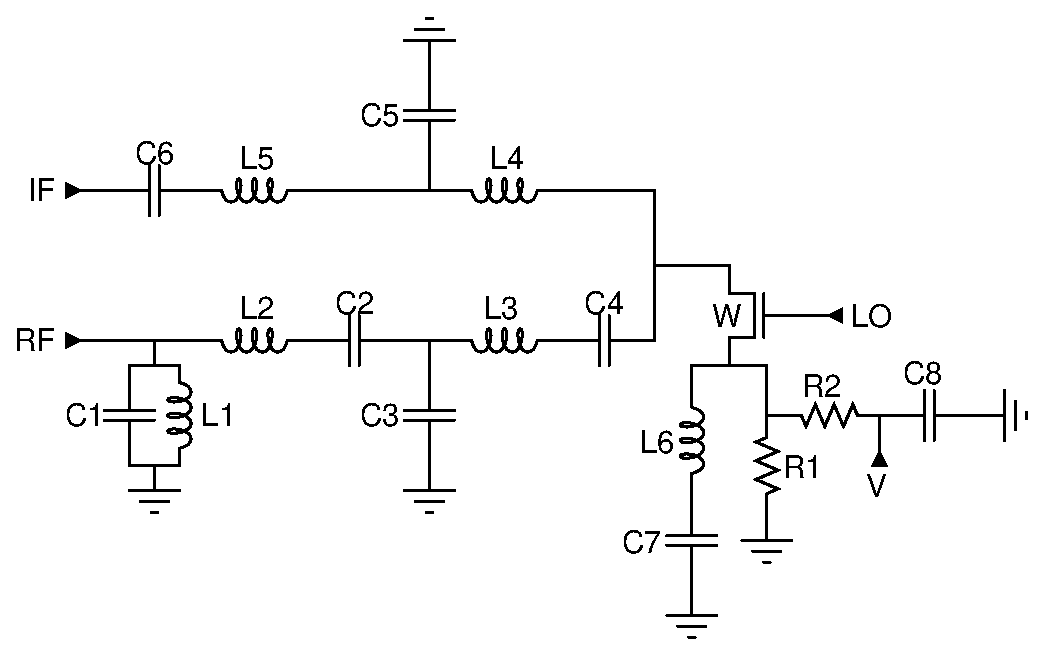
\includegraphics[width=1.0\textwidth]{fig/schematics/sch_mixer_labels}
			\caption[Mixer schematic.]{Schematic of the mixer.}\label{fig:mixerschematicdet}
		\end{figure}

		\begin{table}[h!]
			\caption[Mixer component values.]{Values of the components in the mixer. $W$=\unit[8$\times$75]{\mum} and $V=\unit[5]{V}$.}
			\label{tab:mixerschvalues}
			\centering
			\begin{tabular}{llllll}
				\multicolumn{2}{l}{Capacitors (pF)} & \multicolumn{2}{l}{Inductances (nH)} & \multicolumn{2}{l}{Resistors ($k\Omega$)} \\\hline
				$C_1$ & 1.75 & $L_1$ & 1.0 & $R_1$ & 1.17 \\
				$C_2$ & 8.5 & $L_2$ & 3.6 & $R_2$ & 5.0 \\
				$C_3$ & 0.72 & $L_3$ & 3.2 &  & \\
				$C_4$ & 6.4 & $L_4$ & 5.6 &  & \\
				$C_5$ & 1.4 & $L_5$ & 5.6 &  & \\
				$C_6$ & 5.7 & $L_6$ & 0.1 &  & \\
				$C_7$ & 6.0 &  &  &  & \\
				$C_8$ & 5.0 &  &  &  &
			\end{tabular}
		\end{table}
		
	\newpage
	
	\section{Amplifier LO}
		The LO-amplifier's schematic and component values are found in \autoref{fig:sch_lo_labeled} and \autoref{tbl:sch_lo_values} respectively.
		
		\begin{figure}[hbt!]
			\centering
			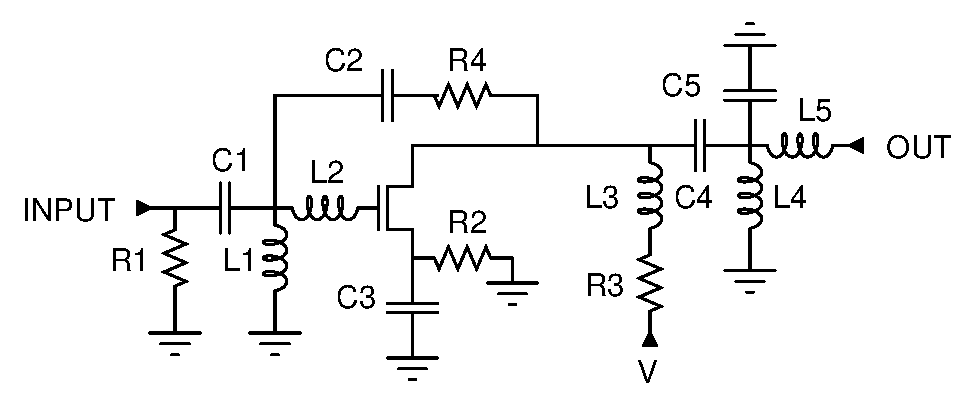
\includegraphics[width=0.8\textwidth]{fig/amplifiers/lo/sch_lo_labeled}
			\caption[Amplifier LO schematic.]{Schematic of the LO-amplifier.}\label{fig:sch_lo_labeled}
		\end{figure}

		\begin{table}[hbt!]
			\caption[LO-amplifier component values.]{Values of the components in LO-amplifier. FET-size is \unit[4$\times$50]{\mum} and $V=\unit[5]{V}$.}
			\label{tbl:sch_lo_values}
			\centering
			\begin{tabular}{llllll}
				\multicolumn{2}{l}{Capacitors (pF)} & \multicolumn{2}{l}{Inductances (nH)} & \multicolumn{2}{l}{Resistors ($\Omega$)} \\\hline
				$C_1$ &  4.0 & $L_1$ & 1.7 & $R_1$ & 300 \\
				$C_2$ &  1.0 & $L_2$ & 1.0 & $R_2$ & 25 \\
				$C_3$ &  6.0 & $L_3$ & 2.8 & $R_3$ & 160 \\
				$C_4$ &  2.3  & $L_4$ & 4.0& $R_4$ & 500 \\
				$C_5$ &  0.65 & $L_5$ & 2.2 &  & 
			\end{tabular}
		\end{table}	

	\newpage	
	
	\section{Amplifier IF1}\label{sec:detif1sch}
		Amplifier IF1 schematic and component values are found in \autoref{fig:if1schematicdet} and \autoref{tab:if1schvalues} respectively.
		
		\begin{figure}[hbt!]
			\centering
			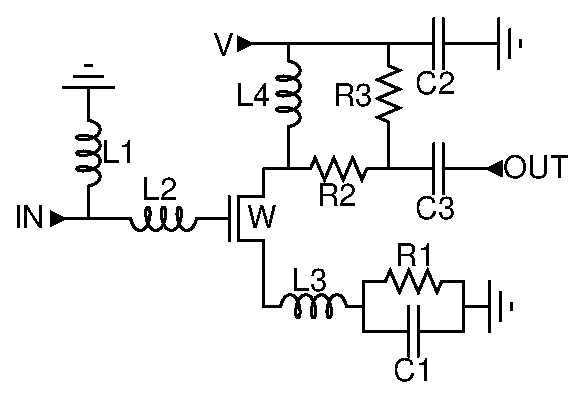
\includegraphics[width=0.7\textwidth]{fig/schematics/sch_if1_labels}
			\caption[Amplifier IF1 schematic.]{Schematic of amplifier IF1.}\label{fig:if1schematicdet}
		\end{figure}

		\begin{table}[hbt!]
			\caption[Amplifier IF1 component values.]{Values of the components in amplifier IF1. $W$=\unit[8$\times$75]{\mum} and $V=\unit[5]{V}$.}
			\label{tab:if1schvalues}
			\centering
			\begin{tabular}{llllll}
				\multicolumn{2}{l}{Capacitors (pF)} & \multicolumn{2}{l}{Inductances (nH)} & \multicolumn{2}{l}{Resistors ($\Omega$)} \\\hline
				$C_1$ & 25  & $L_1$ & 7.1 & $R_1$ & 9.0 \\
				$C_2$ & 7.0 & $L_2$ & 5.6 & $R_2$ & 27 \\
				$C_3$ & 5.0 & $L_3$ & 0.7 & $R_3$ & 130 \\
					  &     & $L_4$ & 4.0 &  &
			\end{tabular}
		\end{table}

	\newpage
	\section{Amplifier IF2}\label{sec:detif2sch}
		Amplifier IF2 schematic and component values are found in \autoref{fig:if2schematicdet} and \autoref{tab:if2schvalues} respectively.
		\begin{figure}[hbt!]
			\centering
			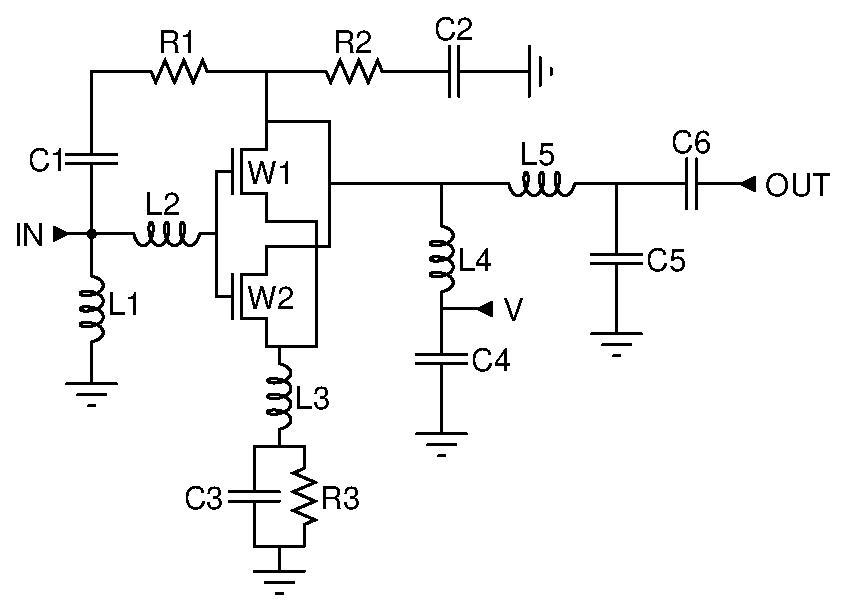
\includegraphics[width=0.8\textwidth]{fig/schematics/sch_if2_labels}
			\caption[Amplifier IF2 schematic.]{Schematic of amplifier IF2.}\label{fig:if2schematicdet}
		\end{figure}

		\begin{table}[hbt!]
			\caption[Amplifier IF2 component values.]{Values of the components in amplifier IF2. $W_1=W_2$=\unit[6$\times$75]{\mum} and $V=\unit[5]{V}$.}
			\label{tab:if2schvalues}
			\centering
			\begin{tabular}{llllll}
				\multicolumn{2}{l}{Capacitors (pF)} & \multicolumn{2}{l}{Inductances (nH)} & \multicolumn{2}{l}{Resistors ($\Omega$)} \\\hline
				$C_1$ & 5.0  & $L_1$ & 5.9 & $R_1$ & 450 \\
				$C_2$ & 5.0  & $L_2$ & 3.2 & $R_2$ & 110 \\
				$C_3$ & 10   & $L_3$ & 0.3 & $R_3$ & 4.2 \\
				$C_4$ & 12   & $L_4$ & 3.5 &  & \\
				$C_5$ & 0.84 & $L_5$ & 0.91 &  & \\
				$C_6$ & 5.0  &       &      &  &
			\end{tabular}
		\end{table}
	
	\newpage
	
		

		
%		\begin{table}[h!]
%			\caption[Level shifter component values.]{Values of the components in the level-shifter. }
%			\label{tab:levelshifterschvalues}
%			\centering
%			\begin{tabular}{ll}
%				\multicolumn{2}{l}{Resistors ($k\Omega$)} \\\hline
%				$R_1$ & 1.6 \\
%				$R_2$ & 2.4 \\
%				$R_3$& 4.0 \\
%				$R_4$& 8.0 \\
%				$R_5$& 8.0 \\
%				$R_6$& 4.8 \\
%				$R_7$ & 5.0
%			\end{tabular}
%		\end{table}